%===============================================================================
% Smile Selenium introduction
%===============================================================================
\newpage{}
\chapter{Introduction}

\section{Le but du projet}

L'intégration continue est un point très important dans le développement d'application pour limité
les bugs. On améliore ainsi la qualité des projets et facilite grandement les livraisons. 

\youTestIt{} fait partie des outils d'intégration continue, en permettant de tester les actions que les
utilisateurs feront sur l'application. Il permet de gérer les campagnes de tests ainsi que de l'automatiser.
L'automatisation des tests se fait via Selenium \footnote{Selenium est un outils permettant l'écriture et
l’exécution de tests sur un navigateur web}. 


\youTestIt{}  est une application WEB, cela permettant un déploient simplifier et un travail en équipe bien
plus simple. La création et la maintenance des tests Selenium peut rapidement devenir très complexe,
il est nécessaire d'avoir un outils facilitant ce processus.

\youTestIt{} a deux objectifs principaux :
\begin{itemize}
	\item Facilité la création et maintenance des tests Selenium  en apportant une approche fonctionnelle.
	\item D'aider à mesurer la qualité d'un projet.
\end{itemize}



Les clients sont rarement des développeurs expérimenter, ils ont besoin d'un outils
qui leurs permettent de concevoir des tests d'un point de vue fonctionnel, et ceux
sans que les contraintes techniques ne freinent leurs taches. 

Cette outils permet également d'améliorer la relation cliente, en les faisant participer
à la vie du projet (descriptions et conceptions de tests Selenium), ou en leurs donnant 
une meilleure vision de l'évolution de la qualité de leurs projets. 

Un point qui est souvent complexe et couteux en temps est le fait de tester un projet 
sur les différents navigateurs cibles.  Le fait d'avoir un outils qui est capable d'exécuter
des tests sur différents plateformes avec une configuration simple est un réel avantage.
Selenium permet de lancer des tests sur différents systèmes d'exploitations et navigateurs, 
cependant la configuration n'est pas simple pour des personnes n'ayant pas des notions 
d'administration système. 

La parallélisation des calculs est également un point important.  Un test Selenium prend du 
temps à s'exécuter. Imaginons que l'on ait  beaucoup de tests avec différents navigateurs, le
temps nécessaire sera conséquent. En distribuant les calculs sur différents machines, le temps
nécessaire pour effectuer l'ensemble de ces tests sera considérablement réduit. 

\begin{description}
	\item \positif{}
	  Approche fonctionnelle des tests Selenium, ne nécessite pas de connaissant approfondie en développement.
	\item \positif{}  Gestion des tests Selenium simplifié.
	\item \positif{}  Tests sur différents environnements plus simple à configurer.
	\item \positif{}  Meilleur vision de l'évolution de la qualité d'un projet (statistiques plus complètes).
	\item \positif{}  Évite les régressions, extrêmement important dans le cadres de TMA.
	\item \positif{}  Améliore la relation clients (participation à la création des tests et ou meilleur vision de la qualité du projet)
\end{description}


%===============================================================================
% Qu'est-ce que Selenium
%===============================================================================
\section{Qu'est-ce que Selenium}
Pour comprendre d'avantage le fonctionnement de \youTestIt{}, il faut comprendre qu'est-ce que
c'est que les tests Selenium.

Selenium est un outils qui permet d'effectuer des tests sur l'interface d'une application Web. Il 
est divisé en deux parties :

\textbf{Selenium IDE}

		C'est un plugin pour Firefox permettant de concevoir les tests. Lors qu'Il est actif il enregistre
		les différentes actions que réalise un utilisateur sur le navigateur.
		\begin{figure}[!h]
     		\begin{center}
			      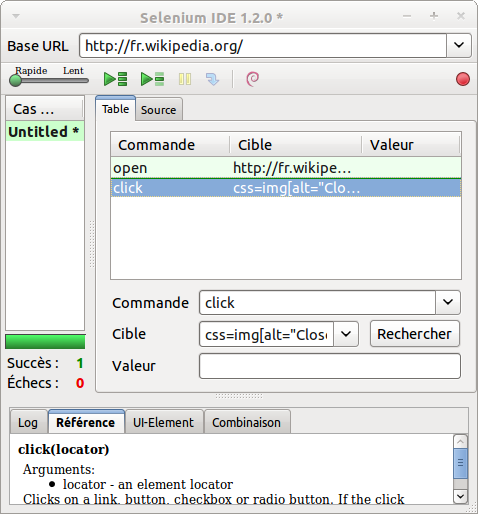
\includegraphics[width=0.3\textwidth]{seleniumIDE}
			      \caption{Interface de Selenium IDE}
			      \label{seleniumIDE}
		    \end{center}
		\end{figure}		
		

\newpage
\textbf{Selenium RC}

		Selenium RC permet d'exécuter des tests Selenium en dehors du plugin firefox. C'est une
		application Java à l'intérieur d'un serveur Jetty qui interprète les différentes commandes Selenium.
		Dans une plateforme d'intégration continue c'est Selenium RC qui est chargé d'effectuer les tests.
		Selenium RC permet également de distribuer l'exécutions des tests sur divers machines. Cependant
		la configuration du Hub\footnote{Le Hub Selenium est le serveur Selenium RC principal dédié à la gestion
		des autres machines.} et des différents nodes\footnote{Les différentes machines liées au Hub Selenium sont
		nommées nodes, ou nœud en français.} se fait en ligne de commandes. Cela demande donc quelques notions
		d'aministration système.
		\begin{figure}[!h]
     		\begin{center}
			      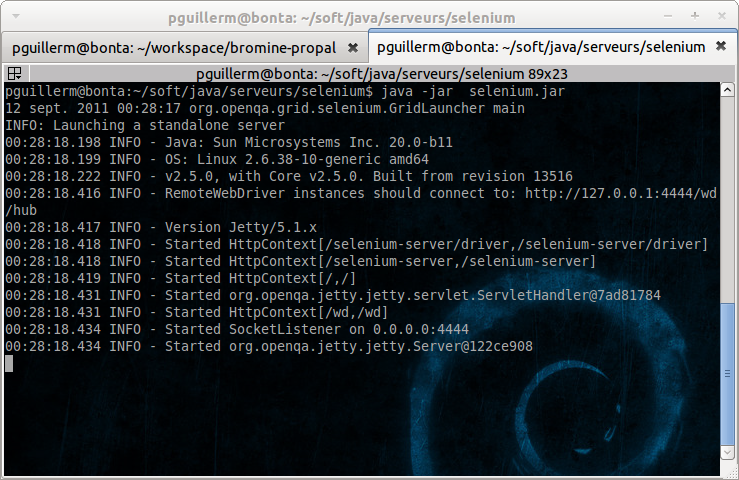
\includegraphics[width=0.4\textwidth]{seleniumRC}
			      \caption{Selenium Remote control}
			      \label{seleniumRC}
		    \end{center}
		\end{figure}	

 		


Ces outils permettent une première approche vis à vis des tests d'intégration. Leurs intégrations n'est pas simple, elle nécessite une bonne connaissance en Maven\footnote{Maven est une application gérant la compilation d'application Java} et
en administration système. 

